
\documentclass[10pt,fleqn, twocolumn]{IEEEtran}
\usepackage{amsfonts}
\usepackage{amsthm}
\usepackage{amsmath}
\usepackage{graphicx}
\usepackage{fancyhdr}


\newtheorem{Prop}{Proposition}
\newtheorem{lemma}{Lemma}
\newtheorem{theorem}{Theorem}

\setlength{\parindent}{3em} \setlength{\oddsidemargin}{0in}
\setlength{\textwidth}{6.5in} % sets 1in left and right margins
\setlength{\topmargin}{0.20in} % change to 0.2in for regular latex
%\setlength{\headheight}{0in}
%\setlength{\footheight}{0.5in}
\setlength{\footskip}{0.5in}
\setlength{\textheight}{9.0in} %sets 1in top and bottom margins
\renewcommand{\baselinestretch}{1} %set to 1.5 for double spacing.

\newcommand{\br}{{\mathbf r}}
\newcommand{\bA}{{\mathbf A}}
\newcommand{\ba}{{\bf a}}
\newcommand{\bb}{{\bf b}}
\newcommand{\bc}{{\bf c}}
\newcommand{\bC}{{\bf C}}
\newcommand{\bd}{{\bf d}}
\newcommand{\be}{{\bf e}}
\newcommand{\bE}{{\bf E}}
\newcommand{\bbf}{{\bf f}}
\newcommand{\bF}{{\bf F}}
\newcommand{\bh}{{\bf h}}
\newcommand{\bH}{{\bf H}}
\newcommand{\bg}{{\bf g}}
\newcommand{\bG}{{\bf G}}
\newcommand{\bq}{{\bf q}}
\newcommand{\bs}{{\bf s}}
\newcommand{\bm}{{\bf m}}
\newcommand{\bn}{{\bf n}}
\newcommand{\bu}{{\bf u}}
\newcommand{\bv}{{\bf v}}
\newcommand{\bw}{{\bf w}}
\newcommand{\bx}{{\bf x}}
\newcommand{\by}{{\bf y}}
\newcommand{\bz}{{\bf z}}
\newcommand{\bL}{{\bf L}}
\newcommand{\bM}{{\bf M}}
\newcommand{\bN}{{\bf N}}
\newcommand{\bS}{{\bf S}}
\newcommand{\bT}{{\bf T}}
\newcommand{\bD}{{\bf D}}
\newcommand{\bX}{{\bf X}}
\newcommand{\bP}{{\bf P}}
\newcommand{\bQ}{{\bf Q}}
\newcommand{\bI}{{\bf I}}
\newcommand{\bR}{{\bf R}}
\newcommand{\bU}{{\bf U}}
\newcommand{\bV}{{\bf V}}
\newcommand{\bW}{{\bf W}}
\newcommand{\bY}{{\bf Y}}
\newcommand{\bZ}{{\bf Z}}
\newcommand{\bJ}{{\bf J}}
\newcommand{\bB}{{\bf B}}
\newcommand{\bzero}{{\bf 0}}
\newcommand{\bgamma}{{\mbox {\boldmath $\gamma$}}}
\newcommand{\btheta}{{\mbox {\boldmath $\theta$}}}
\newcommand{\bvartheta}{{\mbox {\boldmath $\vartheta$}}}
\newcommand{\bDelta}{{\mbox {\boldmath $\Delta$}}}
\newcommand{\bLambda}{{\mbox {\boldmath $\Lambda$}}}
\newcommand{\bPsi}{{\mbox {\boldmath $\Psi$}}}
\newcommand{\bPhi}{{\mbox {\boldmath $\Phi$}}}
\newcommand{\bcA}{{\mbox {\boldmath ${\cal A}$}}}
\newcommand{\bcB}{{\mbox {\boldmath ${\cal B}$}}}
\newcommand{\bcC}{{\mbox {\boldmath ${\cal C}$}}}
\newcommand{\bcD}{{\mbox {\boldmath ${\cal D}$}}}
\newcommand{\bcF}{{\mbox {\boldmath ${\cal F}$}}}
\newcommand{\bcG}{{\mbox {\boldmath ${\cal G}$}}}
\newcommand{\bcL}{{\mbox {\boldmath ${\cal L}$}}}
\newcommand{\bcN}{{\mbox {\boldmath ${\cal N}$}}}
\newcommand{\bcR}{{\mbox {\boldmath ${\cal R}$}}}
\newcommand{\bcS}{{\mbox {\boldmath ${\cal S}$}}}
\newcommand{\bcH}{{\mbox {\boldmath ${\cal H}$}}}
\newcommand{\bcI}{{\mbox {\boldmath ${\cal I}$}}}
\newcommand{\bcO}{{\mbox {\boldmath ${\cal O}$}}}
\newcommand{\bcP}{{\mbox {\boldmath ${\cal P}$}}}
\newcommand{\bcQ}{{\mbox {\boldmath ${\cal Q}$}}}
\newcommand{\bcV}{{\mbox {\boldmath ${\cal V}$}}}
\newcommand{\bcW}{{\mbox {\boldmath ${\cal W}$}}}


\title{MIMO Relay with Finite-Rate Feedback and Imperfect Channel Estimation}
\author{LGE Mobile Research\\San Diego, CA 92131}
\date{}
\begin{document}
\maketitle
\begin{abstract}\small
We investigate how finite-rate feedback and imperfect channel
estimation affect the end-to-end throughput of multi-antenna relay
network in this paper. We start from multi-antenna beamforming
transmission using uniform random codebook and formulate average
SNR loss due to quantization error and imperfect channel
estimation. Following that, we extend our analysis to MIMO relay
network with multiple relay nodes and discuss how the relay
channel capacity is scaled with MIMO pilot channel size, codebook
size and the number of relays. Computer simulations are also
provided to support our results.
\end{abstract}

\section{Introduction}
Multi-antenna systems have received much attention for the past
decade or so, due to their promise of higher spectrum efficiency
with no transmit power increase. Combining wireless relay with
multi-antenna transceiver is essential not only to provide
comprehensive coverage but also to help relieve co-channel
interference in existing wireless systems. For multiple-input
multiple-output (MIMO) transmission, it is well-known that their
performance and complexity can be improved by making channel state
information (CSI) available at the transmitter. This is usually
achieved through a special reverselink CSI feedback channel from
the receiver. For example, there are HS-DPCCH and R-CQI channels
for 3GPP HSPA and 3GPP2 UMB, respectively. In practice, the CSI
received by the transmitter is imperfect since it suffers from
various impairments and limitations, which include round-trip
delay, channel estimation errors, limited codebook, etc. Therefore
the actual link throughput can be much lower in MIMO systems with
feedback. This kind of degradation may be more serious if the
end-to-end capacity is considered for multi-hop MIMO relay
network.

Multi-antenna systems with quantized feedback have been
intensively investigated since 1990s~\cite{Gerlach94}. MIMO
channel quantization as well as codebook design basically is a
Voronoi decomposition problem. It generally is NP-hard. For
uniformed channel distribution, the Voronoi region is
upper-bounded by disk-covering circle and lower-bounded by
sphere-packing boundary. Both of them are open problems in
general. Optimal quantization and feedback for multi-antenna
system is studied in~\cite{Skog03,Lau04}. A MISO/MIMO system with
perfect CQI and Lloyd vector quantization (VQ) is firstly
investigated in~\cite{Narula98} and then with Rayleigh fading
channels in~\cite{Mukka03}. It is linked to Grassmannian line
packing problem in~\cite{Love02}. Lloyd VQ for MIMO codebook
design was also investigated in~\cite{PXia04,Roh04} with different
performance metrics. Most of these investigations are done with
the assumption of perfect channel estimation, even though it is
not true in practice. In most existing multi-antenna systems, MIMO
CSI is estimated using forward-link common pilot channels sent by
transmitter. An overview of pilot-assisted transmission can be
found in~\cite{Tong04}. Besides conventional pilot design by TDM,
CDM and OFDM, superimposed pilots (SIP) have recently received
much attention for MIMO channel estimation~\cite{Coldrey06}. In
practice, it is desirable to understand how to balance MIMO pilot
size and codebook size and both of them are key parameters of
multi-antenna systems. And this problem becomes more critical when
a multi-hop MIMO relay network with finite-rate feedback is
considered.

It is known that there is no general solution to optimal MIMO
quantization. In this paper, a heuristic Voronoi boundary is
presented using Hamming bound. It is shown that this heuristic
boundary is also bounded by disk-covering circle and
sphere-packing boundary and they are asymptotically converged
together. For MIMO CSI estimation, both TDM pilots (TMP) and SIP
are considered and the Cramer-Rao lower bound (CRLB) is presented
for channel estimation. After this,

\section{MIMO System Model And Problem Description\label{MIMO_system_model}}

Consider a transmitter with $M$ transmit antennas and a receiver
with $N$ receive antennas. The channel can be represented by the
$N\times M$ matrix $\bH$. The $N\times 1$ received signal $\by$ is

\begin{equation}
\begin{array}{rcl}
\by& = & \bH\bW\bx+\bn
\end{array}\label{Direct_MIMO}
\end{equation}

\noindent where $\bx$ is the transmitted $M\times 1$ signal vector
by the source with $\bR_{\bx}=\mbox{E}\left\{\bx\bx^{\rm
H}\right\}=\frac{P}{M}\bI_{M}$, where $\left[\ast\right]^{\rm H}$
is the Hermitian conjugate operation and $P$ is the total
transmission power, $\bW=\left[\bw_{1}\ \bw_{2}\ \ldots\
\bw_{M}\right]$ is a $M\times M$ MIMO linear beamforming matrix
with each codeword satisfying $\left\|\bw_{m}\right\|_2=1$, and
$\bn\sim{\bcC\bcN}(0, \sigma^2\bI_{N})$ is a complex circular
white Gaussian vector. It is known that the achievable MIMO
channel efficiency is
\begin{equation}
\begin{array}{rcl}
\eta& = & \mbox{log}\left|\bI_{N}+\frac{P}{M}\bH\bW\bW^{\rm
H}\bH^{\rm H}\right|
\end{array},\label{spectral_eff}
\end{equation}
\noindent where $\left|\ast\right|$ denotes the determinant of
matrix $\ast$. And the received signal-to-noise ratio (SNR) of the
$k$th beam is
\begin{equation}
\begin{array}{rcccl}
\rho_{i}&=&\frac{\mbox{var}\left\{\bH\bw_{i}\right\}x_{i}}{\sigma^2}&=&\frac{\lambda_{i}P_{i}}{\sigma^2}
\end{array},\label{SNR_i}
\end{equation}
\noindent where $\mbox{var}\left\{\ast\right\}$ denotes the
variance function of random variable $\ast$, $\lambda_{i}$ denotes
the antenna gain for the $i$th beam, which is the $i$th eigenvalue
of $\bH$. However, (\ref{spectral_eff}) and (\ref{SNR_i}) are the
results with the assumption of perfect CSI available at
transmitter. This is not true in most practical applications.

In reality, the receiver do channel estimation with pilots sent by
transmitter at first. Accuracy of the channel estimator depends on
the pilot design and placement. There are two popular pilot
patterns, time-multiplexed pilots and superimposed pilots,
recently received much attention, which are shown in
Fig.~\ref{pilot_pattern}. based on channel estimation, the
receiver will choose a beamforming vector from the MIMO precoding
codebook which is shared between the receiver and transmitter.
This procedure is called channel quantization. The receiver then
feeds back the chosen precoding index(es) to the transmitter for
the next transmission. The MIMO beamforming codebook $\bcW$ of the
size $2^B$ consists of $M$-dimensional normalized vectors
$\left\{\bw_{1}, ..., \bw_{2^{B}}\right\}$. It usually takes the
receiver $B$ feedback bits for each beamforming stream. The
codebook is usually designed to quantize channel responses with
certain distortion measures~\cite{Narula98}. This procedure is
also related to Grassmannian line packing and spherical packing on
unit sphere $\bcS_{n}\left(1\right)$~\cite{conway96packing}, where
$\bcS_{n}(R)=\left\{\bv:\ \left\|\bv\right\|=R\right\}$ denotes
$(n-1)$-sphere with radius $R$.

\begin{figure}
\center{
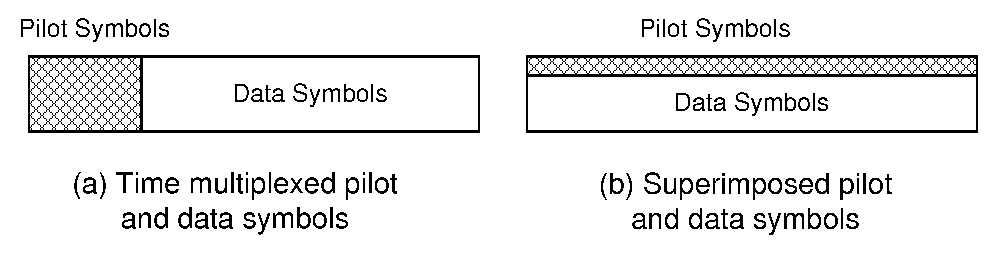
\includegraphics[width=3in, angle=0]{Pilot_Patterns.eps}
\caption{Pilot patterns for channel
estimation.}\label{pilot_pattern} }
\end{figure}

If the codeword $\bw_k$ is chosen to precode signals for $i$th
beam at the transmitter side, there is possible degradation on the
signal received by receiver due to finite-rate feedback and
imperfect channel estimation. This degradation can be expressed by
\begin{equation}
\begin{array}{rcl}
\delta_{i} & = & \min\limits_{\bw\in\bcW}\left\|\bH\bv_{i}-\bH\bw_{k}\right\|\\
&=&\lambda_{i}\left(1-\bv_{i}^{\rm
H}\bw_k\right)-\sum\limits_{j\neq i}\lambda_{j}\bv_{j}^{\rm
H}\bw_{k}
\end{array}\label{delta_i}
\end{equation}

\noindent where $\bv_{i}$ denotes the ideal beamforming vector for
eigen-mode $i$ of $\bH$. It is known that $\delta_{i}$ is one of
the major factors limiting closed-loop MIMO throughput.
$\delta_{i}$ is random variable which depends on $\bv_{i}$,
$\bw_{k}$ and $\lambda_{i}$. There are two items in
(\ref{delta_i}). The first term

\begin{equation}
\begin{array}{rcccl}
\Delta&=&\lambda_{i}\left(1-\bv_{i}^{\rm
H}\bw_k\right)&=&\left(1-\alpha_{i}\right)\lambda_{i}
\end{array}
\end{equation}
\noindent denotes the loss of antenna gain, where

\begin{equation}
\begin{array}{rcl}
\alpha_{i}&=&\bv_{i}^{\rm H}\bw_k
\end{array}.\label{alpha}
\end{equation}

\noindent The second terms

\begin{equation}
\begin{array}{rcccl}
I_{} & = & \sum\limits_{j\neq i}\lambda_{j}\bv_{j}^{\rm
H}\bw_{k}&=&\sum\limits_{j\neq i}\alpha_{j}\bw_{k}
\end{array}\label{IBI}
\end{equation}

\noindent denotes the inter-beam interference (IBI) due to the
correlation between the precoding codeword $\bw_{k}$ and other
eigen-modes $j\neq i$. Since we consider an uniform random
codebook and assume the MIMO channel response $\bH$ is also
uniform random, we can generally get

\begin{equation}\hspace{-0.2in}
\begin{array}{rcccl}
\mbox{E}_{\bH}\left\{\alpha + \sum_{j\neq i}\alpha_{j}\right\}& =
& \alpha + (M-1) \tilde\alpha & = &1
\end{array},\label{alpha_other}
\end{equation}
\noindent where
\begin{equation}
\begin{array}{rcl}
\tilde\alpha&=&\mbox{E}_{j\neq i}\left\{\alpha_{j}\right\}
\end{array}
\end{equation}
\noindent denotes the average interference correlation ratio. With
(\ref{alpha_other}), the average received SNR $\bar\rho_{i}$ for
the $i$th eigen-mode using codeword $\bw_{i}$ can be written by
\begin{equation}
\begin{array}{rcl}
\bar\rho_{i}&=&\mbox{E}_{\bv_{i}\in{\cal
V}_{k}}\left\{\frac{\lambda_{i}\left(\bv_{i}^{\rm
H}\bw_{k}\right)^2P_{i}}{n_{0}^2+ \lambda_{i}\sum\limits_{l\neq
i}^{K}\left(\bv_{i}^{\rm H}\bw_{l}\right)^{2}P_{l}}\right\}\\
&=&\mbox{E}_{\bv_{i}\in{\cal
V}_{k}}\left\{\frac{\alpha_{i}^{2}\rho_{i}}{1+
\lambda_{i}\sum\limits_{l\neq
i}^{K}\frac{\alpha_{l}^{2}}{\lambda_{l}}\rho_{l}}\right\}\\
&\simeq&\frac{\alpha^{2}\rho_{i}}{1+ \lambda_{i}\sum\limits_{l\neq
i}^{K}\frac{\tilde{\alpha}^{2}}{\lambda_{l}}\rho_{l}}\ ,
\end{array}
\end{equation}
\noindent where $K\leq\mbox{min}\left\{M,\ N\right\}$ denotes the
number of beams in use.

\section{Channel Quantization Error}

If the Voronoi decomposition of the codebook $\bcW$ is known, the
correlation ratio $\alpha$ defined in (\ref{alpha}) can be decided
However, the closed-form solution to the boundary of a general
Voronoi cell, which is a polytope, still is open-problem even for
a regular Voronoi tessellation. This makes it difficult to give
some insight of the average SNR $\bar{\rho}_{i}$ for the $i$th
eigen-mode. Instead of finding the exact boundary for $\bcV_{i}$,
we suggest a heuristic approach, in which we use a sphere cap to
approximate the bound by Hamming bound so that the interior of the
sphere cap has the same area as the Voronoi cell. This can be
illustrated in Fig. 2(a). It is known that, for an uniform random
codebook of size $2^{B}$ in $M$-dimensional Euclid space, the area
of a Voronoi cell is given by
\begin{equation}
\begin{array}{rcl}
A\left(\bcV_{k}\right)&=&
\frac{2{\pi}^{M}}{2^{B}\Gamma\left(M\right)}
\end{array}\label{V_area}
\end{equation}
\noindent where $\Gamma\left(\ast\right)$ is the gamma function.
On the other hand, the area of $(m-1)$-complex sphere cap
$\bcC_{m}^{\rm c}\left(\psi,\ R\right)$ with angle $\psi$ and
radius $R$ is
\begin{equation}
\begin{array}{rcl}
A\left(\bcC_{m}^{\rm c}\left(\psi,\
R\right)\right)&=&\Phi_{m}\left(\psi\right)S_{2m}\left(R\right)
\end{array},
\end{equation}
\noindent where $\Phi_{m}\left(\psi\right)$ is defined by
\begin{equation}
\begin{array}{rcl}
\Phi_{m}\left(\psi\right)&=&1-\cos^{(2m-2)}\left(\psi\right)
\end{array}.
\end{equation}
\noindent The examples of sphere and sphere-cap are shown in Fig.
2(b). It can be verified that on a area of a $(m-1)$-complex
sphere $S_{m}^{c}\left(R\right)$ with the radius $R$ is
\begin{equation}
\begin{array}{rcl}
A\left(S_{m}^{c}\left(R\right)\right)&=&A\left(\bcC_{m}^{\rm
c}\left(\pi,\ \bw\right)\right)
\end{array}.
\end{equation}

\begin{figure}
\center{
\includegraphics[width=3.30in, angle=0]{Hamming_Bound.eps}
\caption{Voronoi cell and various bounds}\label{Hamming_bound} }
\end{figure}

\noindent Now the boundary of a Voronoi cell can be approximated
by a hypershpere or a closed space curve decided in the following
proposition.
\begin{Prop}\label{approx_bound} The boundary of the uniform complex Voronoi cell $\bcV_{k}$ can be
approximated by a $(M-1)$-unit complex sphere or a closed complex
space curve.
\begin{equation}\hspace{-0.05in}
\begin{array}{rcl}
\bB\left(\bcV_{k}\right)&\approx& \bcS_{M}^{\rm c}(1)\bigcap \bcL_{M}^{\rm c}(\bw_{k},\ \cos(\theta)) \\
&=&\left\{\bv:\ \left\|\bv\right\|=1,\ \angle\left(\bv,\
\bw_{k}\right)=\theta\right\}\ ,
\end{array}
\end{equation}
\noindent where ${\bcS}_{M}^{\rm c}\left(R\right)$ denotes a
$M$-dimension complex ball in Euclid space with the radius $R$ and
is defined by
\begin{equation}\hspace{-0.2in}
\begin{array}{ll}
{\bcS}_{M}^{\rm c}\left(R\right)=\left\{\bv:\ \left\|\bv\right\|_2=R\right\}=&\\
&\hspace{-1.70in}\left\{\left[x_{m}+iy_{m}\right]_{M\times1}:\
\sum\limits_{m=1}^{M}(x_{m}^2+y_{m}^2)=R^2\right\}\ ,
\end{array}\label{M_complexBall}
\end{equation}
\noindent and $\bcL_{M}^{\rm c}\left(\bw_{k},\
\cos(\theta)\right)=\left\{\bv:\ \bv^{\rm
H}\bw_{k}=\cos(\theta)\right\}$ denotes a complex space curve and
$\theta$ is
\begin{equation}\hspace{-0.00in}
\begin{array}{rcl}
\theta&=&\arccos\left(\alpha_{0}\right)
\end{array}
\end{equation}
\noindent with
\begin{equation}\hspace{-0.00in}
\begin{array}{rcl}
\alpha_{0}&=&\left(\frac{2^B-1}{2^B}\right)^{\frac{1}{2M-2}}
\end{array}
\end{equation}
\noindent denoting the maximum antenna gain loss ratio.
\end{Prop}

On the other hand, it is known that the probability density
function (PDF) $p\left(\alpha\right)$ and the cumulated density
function (CDF) $P\left(\alpha\right)$ of $\alpha$ are
\begin{equation}\hspace{-0.10in}
\begin{array}{rcl}
p\left(\alpha\right)&=&\mbox{Prob}\left\{x=\alpha\right\}\\
&=&\begin{cases}
0 & 0\leq \alpha < \alpha_{0} \\
\frac{\left(2M-2\right)\alpha\left(1-\alpha^2\right)^{M-2}}{\left(1-\alpha_{0}^{2}\right)^{M-1}}
& \alpha_{0}\leq\alpha\leq 1
\end{cases}
\end{array}
\end{equation}
\noindent and
\begin{equation}\hspace{-0.10in}
\begin{array}{rcl}
P\left(\alpha\right)&=&\mbox{Prob}\left\{x\leq\alpha\right\} \\
&=&
\begin{cases}
0 & 0 \leq\alpha < \alpha_{0} \\
1-\left(\frac{1-\alpha^2}{1-\alpha_{0}^2}\right)^{M-1} &
\alpha_{0}\leq\alpha\leq 1
\end{cases}\ .
\end{array}
\end{equation}

With the assumption of uniform random codebook and unform
beam-power distribution, the average received SINR $\bar\rho_{i}$
can be lower-bounded by the following conclusion.
\begin{lemma} The bound of the average received SINR satisfy the
following inequality
\begin{equation}\hspace{-0.10in}
\begin{array}{rcl}
\bar\rho_{i}&\geq& \frac{\sigma_{\alpha}^{2}\rho_{i}}{1+
\frac{1}{M-1}\left(1-\sigma_{\alpha}\right)^{2}\rho_{i}}\ ,
\end{array}
\end{equation}
\noindent where  $\sigma_{\alpha}$ denotes the standard deviation
of $\alpha$ and $\sigma_{\alpha}^2$ given by
\begin{equation}
\begin{array}{rcl}
\sigma_{\alpha}^2&=&\mbox{E}\left\{\alpha_{i}^2\right\}\\
&=&\int\limits_{1}^{\alpha_{0}}\frac{\left(2M-2\right)\alpha^3\left(1-\alpha^2\right)^{M-2}}{\left(1-\alpha_{0}^{2}\right)^{M-1}}d\alpha\\
&=&\frac{1}{M}+\frac{M-1}{M}\alpha_{0}^2\ .
\end{array}
\end{equation}
\end{lemma}

\section{Imperfect Channel Estimation}
The MIMO channel model presented in Section
\ref{MIMO_system_model} is symbol-based without considering
inter-symbol interference (ISI). In general, the channel
estimation model for frequency-selective block fading channel is
different to (\ref{Direct_MIMO}). It shall consider not only the
time-domain spreading of channel impulse response but also the
pilot placement.

\subsection{Data Model and Problem Formulation}
Consider $M$-input and $N$-output channels. The channels are
assumed to be frequency-selective block fading, which means the
random channels taps remain constant for some data packets and
change to independent values for the next. The baseband received
signal can be written as:

\begin{equation}\hspace{-0.20in}
\begin{array}{rcl}
\by(t)&=&\left[\begin{matrix}y_{1}(t)&y_{2}(t)&\cdots&y_{N}(t)\end{matrix}\right]^{\rm T}\\
&=&\left[\begin{matrix}\sum\limits_{m=1}^{M}h_{m,1}(t)\otimes s_m(t)\\ \sum\limits_{m=1}^{M}h_{m,2}(t)\otimes s_m(t)\\ \vdots \\
\sum\limits_{m=1}^{M}h_{m,L}(t)\otimes
s_m(t)\end{matrix}\right]+\bn\\
&=&\left[\begin{matrix}\bh_{1}^{\rm T}(t)\otimes \bs(t)\\ \bh_{2}^{\rm T}(t)\otimes \bs(t)\\ \vdots \\
\bh_{L}^{\rm T}(t)\otimes \bs(t)\end{matrix}\right]+\bn\ ,
% &=&\bH(t)\otimes\bs(t)+\bn \\
\end{array}
\end{equation}
\noindent where $\bh_{l}(t)=\left[h_{1,l}(t)\ h_{2,l}\ \ldots\
h_{M,l}(t)(t)\right]^{\rm T}$ for $t=0,\ 1,\ \ldots\ L_{c}$ is the
channel impulse response vector from the $m$th transmit antenna to
the $L$ receive antenna and $L_{c}$ is the maximum channel order
for all $L$ subchannels. $s_m(t)$ denotes the transmitted symbol
from the $m$th antenna and $n$ represents the independent additive
Gaussian white noise. Due to the commutativity of convolution, the
stretched discrete received signal vector could as well be
expressed by the following expression

\begin{equation}\hspace{-0.00in}
\begin{array}{rcl}
\by&=&\bS\bh+\bn
\end{array},
\end{equation}

\noindent where $\bh$ is the stretched channel response vector
defined by

\begin{equation}\hspace{-0.00in}
\begin{array}{rcl}
\bh&=&\left[\mbox{vec}(\bH_{1})\ \mbox{vec}(\bH_{2})\ \ldots\
\mbox{vec}(\bH_{M})\right]^{\rm T}
\end{array}
\end{equation}
\noindent with $\bH_{k}=\left[\bh_{k}(0)\ \bh_{k}(1)\ \ldots\
\bh_{k}(L_{c}-1)\right]$ and
\begin{equation}\hspace{-0.00in}
\begin{array}{rcl}
\bS&=&\mbox{kron}\left(\left[\bS_{1}\ \bS_{2}\ \ldots\
\bS_{M}\right]^{\rm T},\ \bI\right)
\end{array}
\end{equation}
\noindent with
\begin{equation}\hspace{-0.10in}
\begin{array}{rcl}
\bS_{k}&=&\left[\begin{matrix}
s_{k}(Q)&\cdots&s_{k}(Q-L_{c})\\
s_{k}(Q-1)&\cdots&s_{k}(Q-L_{c}-1)\\
\vdots&\ddots&\vdots\\
s_{k}(1)&\cdots&s_{k}(1-L_{c})
\end{matrix}\right]
\end{array}.
\end{equation}

\subsubsection{Time-Multiplexed Pilot}
The concept of TMP design is to send $Q$ known pilot symbols
first, which is followed by $D$ data symbols. It is shown in
Fig.~\ref{pilot_pattern}. Since the pilot symbols are transmitted
separately from data symbols in time domain, the channel
estimation and data demodulation at the receiver can be much
simplified.

\subsubsection{Superimpose Pilot}

\subsection{Cramer-rao Lower Bound}
The lower bound to the mean-squared errors of unbiased estimates
can be given by the Cramer-Rao bound (CRB), which is defined as
the inverse of the Fisher Information Matrix (FIM). If we denotes
$\bvartheta=\left[\bh^{\rm T}\ \bs_{d}^{\rm T}\right]^{\rm T}$,
the complex FIM is given by

\begin{equation}\hspace{-0.10in}
\begin{array}{rcl}
\mbox{F}\left(\bvartheta\right)&=&\mbox{E}\left\{\left[\frac{\partial\ln\mbox{Pr}\left(\by|\vartheta\right)}{{\partial\vartheta}^{\ast}}\right]\left[\frac{\partial\ln\mbox{Pr}\left(\by|\vartheta\right)}{{\partial\vartheta}^{\ast}}\right]^{\rm H}\right\}\\
 &\hspace{-1.0in}=&\hspace{-0.50in}\sigma_{0}^{-2}\left[\begin{matrix}
\mbox{E}\left\{\bS^{\rm
H}\bS\right\}+\rho_{h}^2\bI&\bzero\\
\bzero&\mbox{E}\left\{\bcH^{\rm H}\bcH\right\}+\rho_{s_{d}}^2\bI
\end{matrix}\right]
\end{array},
\end{equation}
\noindent where
$\rho_{h}^{2}=\mbox{E}\left\{\left|\frac{\partial\ln\mbox{Pr}\left(h\right)}{{\partial
h}^{\ast}}\right|^2\right\}$ and
$\rho_{s_{d}}^{2}=\mbox{E}\left\{\left|\frac{\partial\ln\mbox{Pr}\left(s_{d}\right)}{{\partial
s_{d}}^{\ast}}\right|^2\right\}$.

\subsubsection{Time-Multiplexed Pilot}

\subsubsection{Superimpose Pilot}


\section{Conclusions}

\small
\bibliographystyle{unsrt}
\bibliography{Cooperative_Relay}
\end{document}
